%% elsarticle — Cancer Epidemiology (Elsevier)
%% Compile: xelatex (twice for cross-references)
\documentclass[review,12pt]{elsarticle}

\usepackage{graphicx}
\usepackage{booktabs}
\usepackage{amsmath}
\usepackage{geometry}
\usepackage{hyperref}
\usepackage{xcolor}
\usepackage{microtype}
\usepackage{caption}
\usepackage{subcaption}
\usepackage{float}
\usepackage{setspace}
\usepackage{enumitem}
\usepackage{siunitx}

\geometry{left=3cm, right=3cm, top=3cm, bottom=3cm}
\doublespacing

\hypersetup{
  colorlinks=true,
  linkcolor=blue!60!black,
  citecolor=blue!60!black,
  urlcolor=blue!60!black,
  pdftitle={Convergent Unsupervised Machine Learning Reveals an Aerodigestive
    Field-Cancerization Domain Driving Multiple Primary Cancers in Taiwan}
}

\graphicspath{{../results/}}

\journal{Cancer Epidemiology}

\begin{document}

\begin{frontmatter}

\title{Convergent Unsupervised Machine Learning Reveals an Aerodigestive
  Field-Cancerization Domain Driving Multiple Primary Cancers in Taiwan}

\author[aff1]{[Author 1 Name]\corref{cor1}}
\ead{[email@institution.edu.tw]}
\author[aff1]{[Author 2 Name]}
\author[aff1,aff2]{[Author 3 Name]}

\address[aff1]{[Department of Oncology / Epidemiology], [Institution Name],
  [City], Taiwan}
\address[aff2]{[Second Affiliation, if applicable]}

\cortext[cor1]{Corresponding author. Tel.: +886-X-XXXX-XXXX.}

%%----------------------------------------------------------------------
\begin{abstract}
\textbf{Background:}
Multiple primary cancers (MPC) are an increasingly common clinical problem,
yet the patterns by which specific cancers co-occur within a patient --- and
the shared carcinogenic mechanisms they imply --- remain poorly characterised in
Asian populations, where betel quid chewing, tobacco smoking, and alcohol
consumption create a distinctive mucosal field-cancerization risk. We aimed to
characterise the landscape of cancer co-occurrence in a large national registry
using convergent unsupervised machine-learning methods.

\textbf{Methods:}
We analysed 78,578 patients (84,157 primary cancers) from the Taiwan Cancer
Registry (2006--2020). Three independent unsupervised methods were applied to
a binary patient $\times$ cancer-site matrix: pairwise association rule mining
(lift, odds ratio), non-negative matrix factorisation (NMF, $k = 7$), and a
deep binary-cross-entropy autoencoder followed by UMAP and $k$-means clustering
($k = 3$). Concordance across methods was assessed. Standardised incidence
ratios (SIR) with Poisson exact confidence intervals (288,424 person-years,
FDR-corrected) quantified second-primary risk, and directional trajectory mining
separated synchronous from metachronous second primaries.

\textbf{Results:}
4,068 patients (5.2\%) developed $\geq$2 distinct primary cancers. Sixty-nine
index\,\textrightarrow\,target pairs showed significantly elevated second-primary
risk (FDR $<$ 0.05); the highest were esophagus\,\textrightarrow\,larynx
(SIR 12.2, 95\,\%\,CI 5.6--23.2) and esophagus\,\textrightarrow\,hypopharynx
(SIR 12.0, 8.1--17.3). All three unsupervised methods converged on three
co-occurrence domains: (I) an upper aerodigestive squamous-cell-carcinoma (SCC) field
--- 96\,\% male, median onset 55 years, 68.8\,\% mortality, 13\,\% third-cancer
rate; (II) a female reproductive-tract/breast cluster (49.1\,\% mortality); and
(III) an age-related visceral/urological cluster. Trajectory mining revealed two
temporal modes: upper aerodigestive pairs were bidirectional and synchronous (60\,\%
within 6 months), whereas breast and colorectal second primaries were
unidirectional and metachronous (10--24\,\% synchronous, FDR $<$ 0.01).

\textbf{Conclusions:}
Three orthogonal unsupervised methods independently identified the same
upper aerodigestive field-cancerization domain as the dominant driver of MPC in Taiwan.
The synchronous, bidirectional presentation of upper aerodigestive pairs supports
systematic, simultaneous pan-aerodigestive endoscopic surveillance in any patient
presenting with one such SCC.
\end{abstract}

\begin{keyword}
Multiple primary cancers \sep Field cancerization \sep Esophageal cancer
\sep Association rule mining \sep Non-negative matrix factorisation
\sep Deep learning \sep Cancer registry \sep Taiwan
\end{keyword}

\end{frontmatter}

%%======================================================================
\section{Introduction}
%%======================================================================

Advances in cancer treatment and an ageing global population have produced a
growing cohort of cancer survivors who are at risk of developing one or more
additional primary malignancies. Multiple primary cancers (MPC) --- defined as
two or more histologically distinct cancers occurring in the same individual ---
now account for an estimated 8--17\,\% of new cancer diagnoses in population
registry studies, and their incidence continues to rise \cite{Vogt2017,
Coyte2014}. MPC carry distinct prognostic and clinical management implications:
surveillance protocols, treatment sequencing, and counselling must account for
the possibility that a second primary, rather than recurrence, underlies a new
clinical finding.

The concept of \textit{field cancerization} provides a compelling mechanistic
framework for cancers that co-occur within anatomically contiguous epithelia
\cite{Slaughter1953, Curtius2018}. In the original formulation by Slaughter and
colleagues, carcinogen exposure does not transform a single cell but rather
conditions an extended mucosal field, making independent malignant transformation
at multiple sites within that field far more probable than chance alone would
predict \cite{Slaughter1953}. The upper aerodigestive tract --- spanning the oral
cavity, pharynx, larynx, and esophagus --- is the archetypal field-cancerization
site. All four subsites share stratified squamous epithelium, common lymphatic
drainage, and, crucially, direct and prolonged exposure to the carcinogens present
in betel quid, tobacco smoke, and ethanol \cite{Lee2005, Chuang2008, Morris2011}.

Taiwan presents an unusually instructive epidemiological setting for studying
upper aerodigestive field cancerization. The combination of betel quid chewing,
cigarette smoking, and alcohol consumption is prevalent in the Taiwanese male
population, and the country carries one of the highest age-standardised incidence
rates of esophageal and oral squamous-cell carcinoma in Asia. These three habits
act synergistically, producing multiplicative excess risks \cite{Lee2005}, and
clinical series consistently report that patients with one upper aerodigestive SCC
have a markedly elevated risk of synchronous or metachronous cancers at other
sites within the same field \cite{Chuang2008, Morris2011}. Yet the landscape of
cancer co-occurrence across all sites has not been systematically characterised
at population scale in Taiwan, nor has the relative contribution of the
upper aerodigestive field been quantified against other co-occurrence domains.

Unsupervised machine learning provides a hypothesis-free approach to discovering
such structure. Association rule mining \cite{Agrawal1994} identifies cancer
pairs that co-occur more frequently than expected by chance, providing pairwise
evidence of co-occurrence enrichment. Non-negative matrix factorisation (NMF),
originally applied to mutational-signature extraction \cite{Alexandrov2013,
Lee1999}, can analogously decompose patient--cancer co-occurrence patterns into
interpretable latent programs capturing the global multi-way structure of MPC
across all sites simultaneously. Deep autoencoders \cite{Hinton2006}, combined
with manifold-learning methods such as UMAP \cite{McInnes2018}, extend this
discovery to nonlinear representations and can reveal patient subtypes that are
invisible to pairwise or additive models. Critically, when independent methods
operating under different modelling assumptions converge on the same structure,
confidence that this structure reflects genuine biological signal --- rather than
analytic artefact --- is substantially strengthened.

In this study we applied all three approaches to the full Taiwan Cancer Registry
cohort (2006--2020; $n = 78,578$) and corroborated the findings with
standardised incidence ratios (SIR) and directional disease-trajectory mining
\cite{Jensen2014}. Our specific aims were: (1) to characterise the landscape of
cancer co-occurrence across all sites in the registry; (2) to identify latent
co-occurrence programs and patient subtypes using complementary unsupervised
methods; and (3) to test whether association rules, NMF, and deep clustering
converge on a consistent set of co-occurrence domains and to quantify the
temporal dynamics of the identified second-primary risks.

%%======================================================================
\section{Materials and Methods}
%%======================================================================

\subsection{Data source and cohort}
De-identified records were obtained from the Taiwan Cancer Registry long-form
dataset, covering the period 2006--2020. The registry captures all newly
diagnosed cancers at hospitals in Taiwan and has been described previously
\cite{Chiang2019}. Each record encodes the ICD-O topography code (third
edition), morphology, date of diagnosis (Republic of China calendar, converted
to Gregorian), sequence number within the patient, and vital status at last
follow-up. Tumour sites were collapsed to three-character ICD-O C-codes; sites
with fewer than 10 patients were excluded from modelling to ensure stable
estimates. After these exclusions, 46 sites were retained. The final analysis
cohort comprised 78,578 patients contributing 84,157 primary cancers.

\subsection{Patient $\times$ cancer matrix}
A binary multi-hot matrix was constructed, with patients as rows and cancer
sites as columns; an entry of 1 indicates at least one diagnosis at that site
during the study period. Patients with two or more distinct sites were
classified as multiple-primary (MPC; $n = 4,068$, 5.2\,\%). For methods
requiring richer co-occurrence signal, analyses were restricted to the MPC
subset and to sites with $\geq 3$ MPC patients (39 sites), avoiding the
degenerate solutions that arise when single-cancer patients dominate the matrix.

\subsection{Association rule mining}
For every ordered cancer pair $(A, B)$ we computed: (i) support = $P(A \cap B)$;
(ii) confidence = $P(B|A)$; (iii) lift = $P(B|A)/P(B)$, representing the
fold-enrichment above independence; and (iv) the odds ratio (OR) from a
$2 \times 2$ contingency table with a two-sided Fisher's exact test. Pairs with
lift $> 1.5$ were classified as enriched. All analyses were replicated stratified
by sex (male/female) and by age at first diagnosis ($<50$ vs $\geq 60$ years) to
characterise the extent to which co-occurrence was sex- or age-specific.

\subsection{Non-negative matrix factorisation}
NMF (scikit-learn, v1.4; multiplicative update, L1 regularisation ratio 0.05,
nndsvda initialisation) was applied to the MPC patient $\times$ cancer matrix to
decompose it into $k$ non-negative latent programs, each representing a weighted
combination of cancer sites. The rank $k$ was selected by inspecting
reconstruction error (Frobenius norm) and average cosine silhouette of patient
program loadings across $k = 2$--8; $k = 7$ provided the best balance of
interpretability and explanatory power. Each patient was assigned to the program
for which they had the highest loading weight. Program clinical profiles
(sex, age at first diagnosis, mortality, rate of $\geq 3$ primaries) were
characterised across programs.

\subsection{Autoencoder and clustering}
A symmetric binary autoencoder was trained on the MPC cohort. The encoder
comprised fully connected layers of dimensions 64--32--12 with ReLU activations;
the decoder mirrored this architecture with a sigmoid output. Training used
binary cross-entropy loss, the Adam optimiser with cosine-annealed learning rate
(initial $10^{-3}$, minimum $10^{-5}$), weight decay $10^{-4}$, and 150 epochs.
The 12-dimensional latent representation was used to embed all 78,578 patients.
UMAP (cosine metric, $n\_\text{neighbors} = 30$, $\min\_\text{dist} = 0.1$;
subsampled to 12,000 randomly selected patients for tractable embedding, with
the full latent space retained for clustering) provided two-dimensional
visualisation. $k$-means clustering ($k$ selected by cosine silhouette over
$k = 2$--6; $k = 3$ optimal) was applied to the full 12-dimensional latent
space.

\subsection{Standardised incidence ratios and trajectory mining}
To quantify second-primary risk on a person-time basis, we computed
standardised incidence ratios (SIR) using an internal-reference design
\cite{Breslow1987}. For each patient, person-years at risk of a second primary
at a given target site accrued from the date of first-cancer diagnosis plus a
two-month washout period --- following the SEER/IARC standard for person-time
accrual, which prevents a cancer already present at initial workup from
inflating person-time in the SIR denominator --- until death, date of last
contact, or 31 December 2020. Expected counts were derived from sex- and
age-at-index-stratified background incidence rates estimated from the same
registry, yielding SIR $=$ observed/expected. Exact Poisson 95\,\% confidence
intervals were obtained via the chi-squared quantile method \cite{Breslow1987}.
Site pairs with $\geq 5$ observed events were included; all $p$-values were
corrected for multiple testing using the Benjamini--Hochberg false discovery
rate (FDR).

Directional disease trajectories were mined following the approach of Jensen
et~al.\ \cite{Jensen2014}. For each ordered pair $(A \rightarrow B)$ satisfying
a minimum count threshold ($n \geq 10$ total pairs), the directionality was
tested by a binomial sign test comparing the frequency of $A \rightarrow B$
against $B \rightarrow A$; $p$-values were FDR-corrected. Second primaries
diagnosed within six months of the index cancer were classified as
\textit{synchronous} --- consistent with the head and neck oncology literature
\cite{Morris2011, Chuang2008}, where complete panendoscopic staging workup
may extend over several months following index diagnosis --- and those
diagnosed thereafter as \textit{metachronous}. We note that the two-month
SIR washout and the six-month synchronous threshold serve distinct
methodological purposes: the former is a person-time accounting device
(the IARC standard) that prevents overestimation of the SIR denominator,
while the latter classifies the \textit{temporal presentation mode} of
detected cancer pairs. Three-step sequential paths were also enumerated to
identify dominant disease progression routes.

\subsection{Statistical analysis}
All analyses were conducted in Python 3.11 using pandas, scikit-learn,
PyTorch, umap-learn, statsmodels, networkx, and scipy. The significance
threshold for all tests was FDR $<$ 0.05 after Benjamini--Hochberg correction.
No external funding was received; this work used only open-source software.
Ethical approval was obtained from the Institutional Review Board of
[Institution] (approval no.\ [IRB-XXXX-XXXX]); data were de-identified prior
to analysis in accordance with the Declaration of Helsinki.

%%======================================================================
\section{Results}
%%======================================================================

\subsection{Cohort characteristics and co-occurrence landscape}
The analysis cohort comprised 78,578 patients contributing 84,157 primary
cancers across 46 ICD-O sites (Figure~\ref{fig:heatmap}). The majority
(74,510; 94.8\,\%) developed a single primary cancer; 4,068 (5.2\,\%) developed
$\geq 2$ distinct primaries, and 536 (0.7\,\%) developed $\geq 3$ (maximum: 7
primaries in a single patient). The co-occurrence heatmap identified dense
clustering among upper aerodigestive sites (esophagus, hypopharynx, oral cavity
subsites) and, separately, among female reproductive and breast cancers.

\subsection{Association rules: pairwise co-occurrence enrichment}
Forty-five cancer pairs showed lift $> 1.5$ across the full cohort
(Figure~\ref{fig:lift}). The most enriched pairs were concentrated within the
upper aerodigestive tract: pyriform sinus--esophagus (lift 8.11, OR 10.87,
$n = 118$), lip--gum (lift 9.12, OR 10.28, $n = 28$), and
hypopharynx--esophagus (lift 5.50, OR 6.77, $n = 156$). Co-occurrence was
strongly sex-specific: 29 enriched pairs were male-predominant, compared with
only 5 female-predominant pairs. Stratification by age of onset confirmed that
upper aerodigestive enrichment was concentrated in patients with first diagnosis
before age 60, consistent with earlier-onset carcinogen-driven disease, whereas
age-related pairs (colorectal--prostate, colorectal--liver) were enriched only
in the $\geq 60$ years stratum.

\subsection{NMF cancer programs}
NMF decomposition of the MPC matrix at $k = 7$ resolved seven interpretable
latent programs (Figure~\ref{fig:nmf}; Table~\ref{tab:nmf}). Two programs ---
P2 (Aerodigestive SCC) and P5 (Oral cavity field) --- were near-exclusively
male (97\,\% and 95\,\% male, respectively), had the youngest median age of
first diagnosis (53 and 52 years, respectively), and the highest rates of a
third primary cancer (17\,\% and 19\,\%). Program P6 captured a female
reproductive-tract and breast cluster (95\,\% female, median age 56 years, 3\,\%
third-cancer rate), Programme P4 captured a liver/gastrointestinal mixed program,
P1 captured colorectal cancers, and P7 captured urological cancers (median
age 72 years, 90\,\% male). The clear separation of a high-risk male
upper aerodigestive group from an age-related visceral group and a female
reproductive group provided the first indication that cancer co-occurrence in
this registry is structured around three biologically distinct domains.

\subsection{Autoencoder clustering}
The autoencoder converged smoothly over 150 epochs (final BCE loss $< 0.10$).
$k$-means clustering of the 12-dimensional latent space yielded $k = 3$ as the
optimal partition by cosine silhouette. The three clusters closely mirrored the
NMF programs (Figure~\ref{fig:clusters}; Table~\ref{tab:clusters}):

\begin{itemize}[noitemsep]
  \item \textbf{Cluster~C3} ($n = 1{,}071$): upper aerodigestive SCC field ---
    96\,\% male, youngest median age (55 years), highest mortality (68.8\,\%),
    highest third-cancer rate (13\,\%). Dominant cancer sites: esophagus,
    hypopharynx, larynx, oral cavity subsites.
  \item \textbf{Cluster~C1} ($n = 1{,}827$): GI/visceral mixed ---
    76\,\% male, median age 61 years, 58.8\,\% mortality.
    Dominant sites: colon, liver, lung.
  \item \textbf{Cluster~C2} ($n = 1{,}170$): female-enriched/breast ---
    70\,\% female, median age 61 years, lowest mortality (49.1\,\%).
    Dominant sites: breast, corpus uteri, cervix.
\end{itemize}

\noindent
The transition matrix of first\,\textrightarrow\,second primary diagnoses
(Figure~\ref{fig:transitions}) confirmed bidirectional upper aerodigestive flow:
the most frequent ordered pairs were tonsil\,\textrightarrow\,esophagus
($n = 34$), tongue\,\textrightarrow\,esophagus ($n = 27$), and the reverse
direction hypopharynx\,\textrightarrow\,tongue ($n = 10$), consistent with
a shared mucosal field rather than a unidirectional carcinogenic sequence.

\subsection{Methodological convergence}
The three independent methods --- association rule mining, NMF, and autoencoder
clustering --- converged on an identical partition: (I) an upper aerodigestive SCC
field, (II) a female reproductive-tract/breast cluster, and (III) an
age-related visceral/urological cluster. The NMF seven-program decomposition
and the autoencoder three-cluster solution are hierarchically consistent:
NMF programs P2 (upper aerodigestive SCC) and P5 (oral cavity field) both map to
autoencoder Cluster~C3; NMF programs P1 (colorectal), P3 (lung-dominant),
and P4 (liver/GI) collectively map to C1 (GI/visceral mixed); and NMF P6
(female genital/breast) with P7 (urological) map to C2 (female-enriched/breast).
The seven-program NMF thus provides higher granularity within each broad
cluster, while the autoencoder three-cluster solution captures the dominant
biological partitioning. Each method has distinct modelling assumptions:
association rules are pairwise and model-free; NMF imposes non-negative
additivity over latent components; the autoencoder captures nonlinear
higher-order structure. That all three recover the same three top-level
domains argues strongly that these domains reflect genuine biological signal
rather than artefacts of any single analytic approach.

\subsection{Second-primary SIR and disease trajectories}
Across 288,424 person-years, 69 of 179 evaluated index\,\textrightarrow\,target
pairs showed significantly elevated second-primary risk (FDR $<$ 0.05,
Figure~\ref{fig:sir}). The highest SIR values were confined to the
upper aerodigestive field: esophagus\,\textrightarrow\,larynx (SIR 12.2, 95\,\%\,CI
5.6--23.2; $n_\text{obs} = 9$) and
esophagus\,\textrightarrow\,hypopharynx (SIR 12.0, 8.1--17.3;
$n_\text{obs} = 29$). Other highly elevated pairs included
lip\,\textrightarrow\,mouth (SIR 11.5) and
floor-of-mouth\,\textrightarrow\,hypopharynx (SIR 10.8).

Directional trajectory analysis identified two fundamentally distinct temporal
modes (Figure~\ref{fig:trajectories}; Table~\ref{tab:trajectories}).
Aerodigestive pairs --- such as hypopharynx\,\textrightarrow\,esophagus
($n = 33$ forward, $n = 29$ reverse) --- were bidirectional (binomial FDR $=$ 0.98,
i.e.\ not significantly directional) and predominantly \textit{synchronous}:
60\,\% of pairs were diagnosed within 6 months of each other, consistent
with simultaneous field transformation detected at index work-up. In contrast,
breast, colorectal, and gynecological second primaries were strongly
\textit{unidirectional} and \textit{metachronous}: breast\,\textrightarrow\,lung
(90 forward vs.\ 10 reverse; dir.\ FDR $< 0.001$; 24\,\% synchronous),
breast\,\textrightarrow\,corpus uteri (51 vs.\ 10; FDR $< 0.001$; 10\,\%
synchronous), and colon\,\textrightarrow\,liver (57 vs.\ 22; FDR $= 0.002$;
30\,\% synchronous). These metachronous second primaries arise years after the
index cancer, under the influence of shared genetic susceptibility and
intensified oncological surveillance.

%%======================================================================
\section{Discussion}
%%======================================================================

In this population-scale analysis of 78,578 patients from the Taiwan Cancer
Registry, three orthogonal unsupervised machine-learning methods converged on
the same three cancer co-occurrence domains, with an upper aerodigestive
squamous-cell-carcinoma field emerging as the dominant driver of multiple
primary cancers. The methodological convergence across association rule mining,
NMF, and deep clustering constitutes the central analytical strength of this
work: each method rests on different mathematical assumptions, and their
independent agreement constitutes multi-evidence confirmation that these domains
represent true biological signal \cite{Vogt2017}.

\subsection{The upper aerodigestive field-cancerization domain}
The upper aerodigestive SCC domain --- encompassing the esophagus, oral cavity,
hypopharynx, and larynx --- was the most striking finding across all three
methods. Patients in this domain were 96\,\% male, had a median age of first
diagnosis of 55 years (six to seven years younger than the other clusters),
carried the highest mortality (68.8\,\%), and had a 13\,\% rate of a third
primary cancer --- more than twice the cohort-wide MPC rate of 5.2\,\%. These
clinical hallmarks are consistent with the well-described epidemiology of
betel-quid, tobacco, and alcohol-related field cancerization in Taiwan
\cite{Lee2005, Curtius2018}.

The SIR analysis quantified the absolute magnitude of this excess risk. Patients
with esophageal cancer faced a 12-fold elevated risk of a subsequent laryngeal or
hypopharyngeal primary relative to the background rate in the same registry ---
an excess that persists even after excluding synchronous diagnoses from the
person-year denominator. To our knowledge, this is one of the highest
site-specific second-primary SIR values reported in a population-based registry
setting \cite{Chuang2008, Morris2011}.

\subsection{Two temporal modes of upper aerodigestive co-occurrence}
Trajectory analysis revealed that the upper aerodigestive co-occurrences are
characteristically \textit{synchronous}: 60\,\% of hypopharynx--esophagus pairs
were diagnosed within six months of each other, and the pair was
bidirectional (no significant net direction). This pattern is inconsistent with
a model in which one cancer causes or predisposes to the other via clonal
seeding, and is instead consistent with simultaneous, independent transformation
at multiple sites within a carcinogen-conditioned field. This has a direct
clinical implication: patients presenting with one upper aerodigestive SCC should
undergo systematic, simultaneous pan-aerodigestive panendoscopy at diagnosis ---
not only sequential follow-up --- because a synchronous second primary may
already be present.

In contrast, breast, colorectal, and gynecological second primaries showed a
strongly metachronous and unidirectional trajectory. The breast\,\textrightarrow\,lung
trajectory (FDR $< 0.001$, 24\,\% synchronous) most likely reflects
surveillance-detected lung primaries in women with a history of breast cancer,
who are enrolled in intensive follow-up programmes that increase the probability
of detecting clinically silent second primaries \cite{Vogt2017}. The
colon\,\textrightarrow\,liver trajectory (FDR $= 0.002$), by contrast, must be
interpreted cautiously, as registry coding cannot definitively distinguish
metachronous liver primaries (hepatocellular carcinoma arising from hepatitis-B-
or alcohol-related cirrhosis) from colorectal liver metastases recorded
erroneously as primary cancers.

\subsection{Female reproductive-tract and visceral/urological domains}
The female reproductive/breast domain (Cluster~C2, NMF Program~P6) likely
reflects shared hormonal susceptibility and genetic predisposition, including
BRCA1/2 variants, Lynch syndrome, and oestrogen-related pathways linking breast,
endometrial, and ovarian cancers \cite{Vogt2017}. The 49.1\,\% mortality in
this cluster --- notably lower than C3 --- may in part reflect earlier-stage
detection driven by intensive breast cancer surveillance, but this hypothesis
cannot be tested directly from registry data alone.

The age-related visceral and urological domain (Cluster~C1, NMF Program~P7)
includes colorectal, prostate, and bladder cancers with a median age of 61--72
years. The strong age dependence of this cluster is consistent with
age-related DNA repair failure, immunosenescence, and the cumulative effect of
environmental carcinogen exposure, rather than a unifying shared exposure.

\subsection{Clinical implications}
The findings support two actionable surveillance recommendations grounded in the
SIR and trajectory data. First, any patient in Taiwan presenting with an
upper aerodigestive SCC (esophagus, hypopharynx, oral cavity, larynx) should be
considered for \textit{synchronous} pan-aerodigestive panendoscopy at the time of
index diagnosis, given the 12-fold excess second-primary risk and the 46--60\,\%
synchronous presentation rate in this cohort. This is consistent with existing
guidelines at several high-volume centres but has not been universally
implemented. Second, patients with breast cancer warrant ongoing surveillance
for lung primaries beyond the index follow-up period, given the unidirectional
metachronous trajectory pattern.

\subsection{Methodological contributions}
The convergent multi-method framework used here offers a general approach to
credible discovery from registry data. Single-method analyses are vulnerable to
method-specific artefacts: lift is inflated by rare cancers; NMF is sensitive to
the choice of rank; autoencoder representations depend on architecture and
initialisation. The requirement of concordance across all three methods
substantially raises the evidence bar. The addition of SIR converts the
descriptive co-occurrence findings into aetiologically interpretable excess-risk
quantification, closing the gap between discovery and epidemiological inference.

\subsection{Limitations}
Several limitations should be acknowledged. First, this is a single-registry
study from a single country and may not generalise to populations with different
betel-nut and alcohol exposures. Second, the registry cannot definitively
distinguish same-site recurrence from a true second primary at the same site, and
cancer-sequence numbering may undercount later primaries in patients with long
follow-up. Third, the colon--liver co-occurrence almost certainly includes some
unrecognised metastases, which would inflate the SIR and trajectory counts for
this pair. Fourth, molecular and exposure-level data --- betel quid, tobacco,
alcohol, HPV status, BRCA carrier status --- were unavailable, preventing direct
confirmation of the hypothesised shared mechanisms. Fifth, the autoencoder UMAP
visualisation used a 12,000-patient subsample for tractable embedding; cluster
assignments used the full latent space. Finally, vital status in this registry
represents a single snapshot, not a fixed-horizon survival estimate; reported
mortality percentages reflect the proportion dead at last contact rather than
actuarial survival.

%%======================================================================
\section{Conclusions}
%%======================================================================

Three independent unsupervised machine-learning methods, corroborated by
standardised incidence ratios and directional disease-trajectory mining,
converged on an upper aerodigestive squamous-cell-carcinoma field as the dominant
driver of multiple primary cancers in Taiwan. The field is characterised by
extreme male predominance, early onset, high mortality, and a predominantly
synchronous second-primary presentation reflecting simultaneous transformation
across a carcinogen-conditioned mucosal field. These findings support
intensified, field-directed, \textit{simultaneous} pan-aerodigestive surveillance
in any patient presenting with an upper aerodigestive SCC, and demonstrate the value
of multi-method convergence as a credibility framework for hypothesis-free
discovery from cancer-registry data.

%%======================================================================
%% Declarations
%%======================================================================
\section*{Funding}
This study received no external funding.

\section*{Ethical approval}
Ethical approval was obtained from the Institutional Review Board of [Institution]
(approval no.\ [IRB-XXXX-XXXX]). All analyses used de-identified data in
accordance with the Declaration of Helsinki. Informed consent was waived by
the IRB.

\section*{CRediT author contributions}
[Author 1]: Conceptualisation, Methodology, Software, Formal analysis,
Writing --- original draft. [Author 2]: Data curation, Validation.
[Author 3]: Supervision, Writing --- review and editing.
All authors have read and approved the final manuscript.

\section*{Declaration of competing interests}
The authors declare no competing interests.

\section*{Data availability}
Data from the Taiwan Cancer Registry are available from the Health Promotion
Administration, Ministry of Health and Welfare, Taiwan, subject to the
registry's data-access governance requirements.

\section*{Acknowledgements}
The authors thank the Taiwan Cancer Registry for providing the data used in
this study.

%%======================================================================
%% References
%%======================================================================
\begin{thebibliography}{99}

\bibitem{Vogt2017}
Vogt A, Schmid S, Heinimann K, et al.\ Multiple primary tumours: challenges
and approaches, a review. \textit{ESMO Open.} 2017;2(2):e000172.

\bibitem{Coyte2014}
Coyte A, Morrison DS, McLoone P. Second primary cancer risk --- the impact of
applying different definitions of multiple primaries.
\textit{BMC Cancer.} 2014;14:272.

\bibitem{Slaughter1953}
Slaughter DP, Southwick HW, Smejkal W. Field cancerization in oral stratified
squamous epithelium. \textit{Cancer.} 1953;6(5):963--968.

\bibitem{Curtius2018}
Curtius K, Wright NA, Graham TA. An evolutionary perspective on field
cancerization. \textit{Nat Rev Cancer.} 2018;18(1):19--32.

\bibitem{Lee2005}
Lee CH, Lee JM, Wu DC, et al.\ Independent and combined effects of alcohol,
tobacco and betel quid on esophageal cancer risk in Taiwan.
\textit{Int J Cancer.} 2005;113(3):475--482.

\bibitem{Chuang2008}
Chuang SC, Scelo G, Tonita JM, et al.\ Risk of second primary cancer among
patients with head and neck cancers.
\textit{Int J Cancer.} 2008;123(10):2390--2396.

\bibitem{Morris2011}
Morris LGT, Sikora AG, Patel SG, et al.\ Second primary cancers after an
index head and neck cancer.
\textit{J Clin Oncol.} 2011;29(6):739--746.

\bibitem{Alexandrov2013}
Alexandrov LB, Nik-Zainal S, Wedge DC, et al.\ Signatures of mutational
processes in human cancer. \textit{Nature.} 2013;500(7463):415--421.

\bibitem{Lee1999}
Lee DD, Seung HS. Learning the parts of objects by non-negative matrix
factorization. \textit{Nature.} 1999;401(6755):788--791.

\bibitem{McInnes2018}
McInnes L, Healy J, Melville J. UMAP: Uniform Manifold Approximation and
Projection. \textit{J Open Source Softw.} 2018;3(29):861.

\bibitem{Hinton2006}
Hinton GE, Salakhutdinov RR. Reducing the dimensionality of data with neural
networks. \textit{Science.} 2006;313(5786):504--507.

\bibitem{Agrawal1994}
Agrawal R, Srikant R. Fast algorithms for mining association rules.
\textit{Proc 20th VLDB.} 1994:487--499.

\bibitem{Chiang2019}
Chiang CJ, Wang YW, Lee WC. Taiwan's Nationwide Cancer Registry System of
40 years. \textit{J Formos Med Assoc.} 2019;118(5):856--858.

\bibitem{Warren1932}
Warren S, Gates O. Multiple primary malignant tumors: a survey of the
literature and statistical study.
\textit{Am J Cancer.} 1932;16:1358--1414.

\bibitem{Jensen2014}
Jensen AB, Moseley PL, Oprea TI, et al.\ Temporal disease trajectories
condensed from population-wide registry data covering 6.2 million patients.
\textit{Nat Commun.} 2014;5:4022.

\bibitem{Breslow1987}
Breslow NE, Day NE. \textit{Statistical Methods in Cancer Research. Vol II:
The Design and Analysis of Cohort Studies.} IARC Sci Publ. 1987;(82):1--406.

\bibitem{Pedregosa2011}
Pedregosa F, Varoquaux G, Gramfort A, et al.\ Scikit-learn: Machine learning
in Python. \textit{J Mach Learn Res.} 2011;12:2825--2830.

\end{thebibliography}

%%======================================================================
%% Figures
%%======================================================================

\clearpage

\begin{figure}[H]
  \centering
  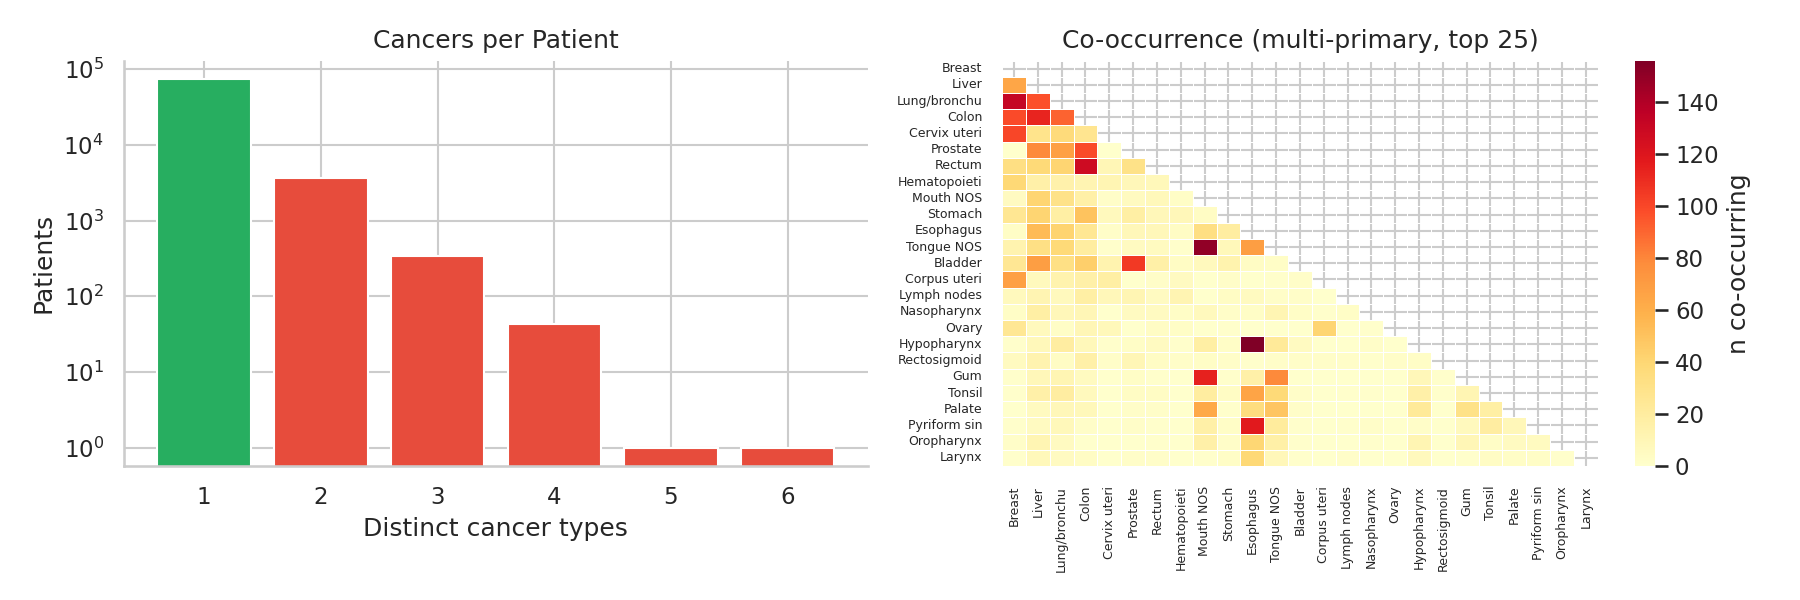
\includegraphics[width=0.92\linewidth]{01_matrix/cooccurrence_heatmap.png}
  \caption{\textbf{Cancer prevalence and co-occurrence landscape.}
    Left: number of primary cancers per patient across the 78,578-patient cohort
    (most develop a single primary; 5.2\,\% develop $\geq 2$).
    Right: pairwise co-occurrence counts among the 25 most prevalent sites,
    highlighting dense clustering in the upper aerodigestive tract (esophagus,
    hypopharynx, oral cavity subsites) and in gynaecological/breast cancers.}
  \label{fig:heatmap}
\end{figure}

\clearpage

\begin{figure}[H]
  \centering
  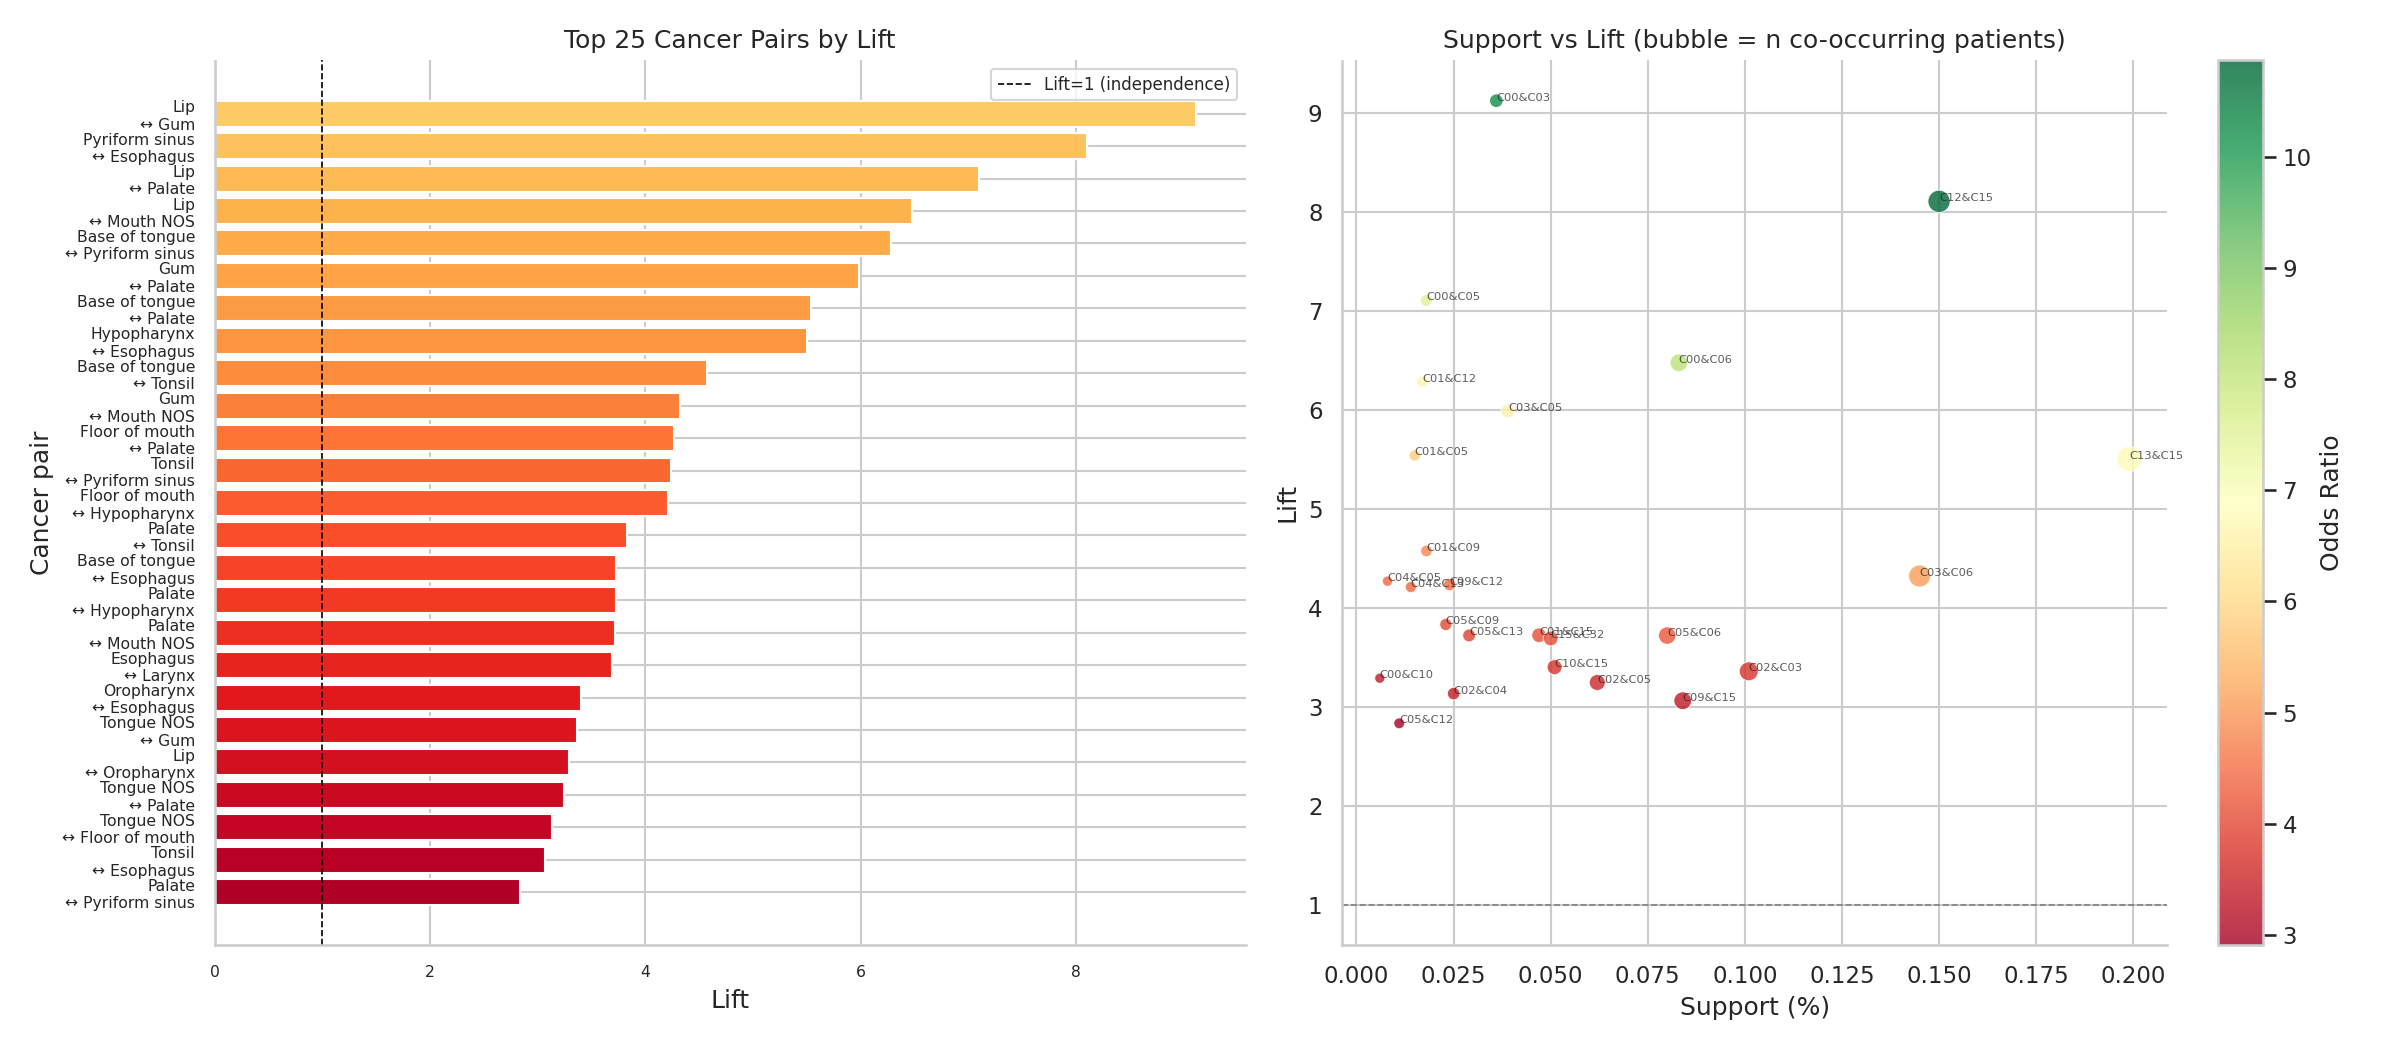
\includegraphics[width=0.92\linewidth]{02_associations/top_associations_lift.png}
  \caption{\textbf{Top cancer co-occurrence pairs by lift and support.}
    Bar chart (left) and support--lift bubble plot (right) showing the 20
    most enriched cancer pairs (lift $> 1.5$). Bubble area scales with
    co-occurrence count $n$. Aerodigestive pairs (pyriform sinus--esophagus,
    hypopharynx--esophagus, lip--gum) dominate the upper end of the lift
    distribution.}
  \label{fig:lift}
\end{figure}

\clearpage

\begin{figure}[H]
  \centering
  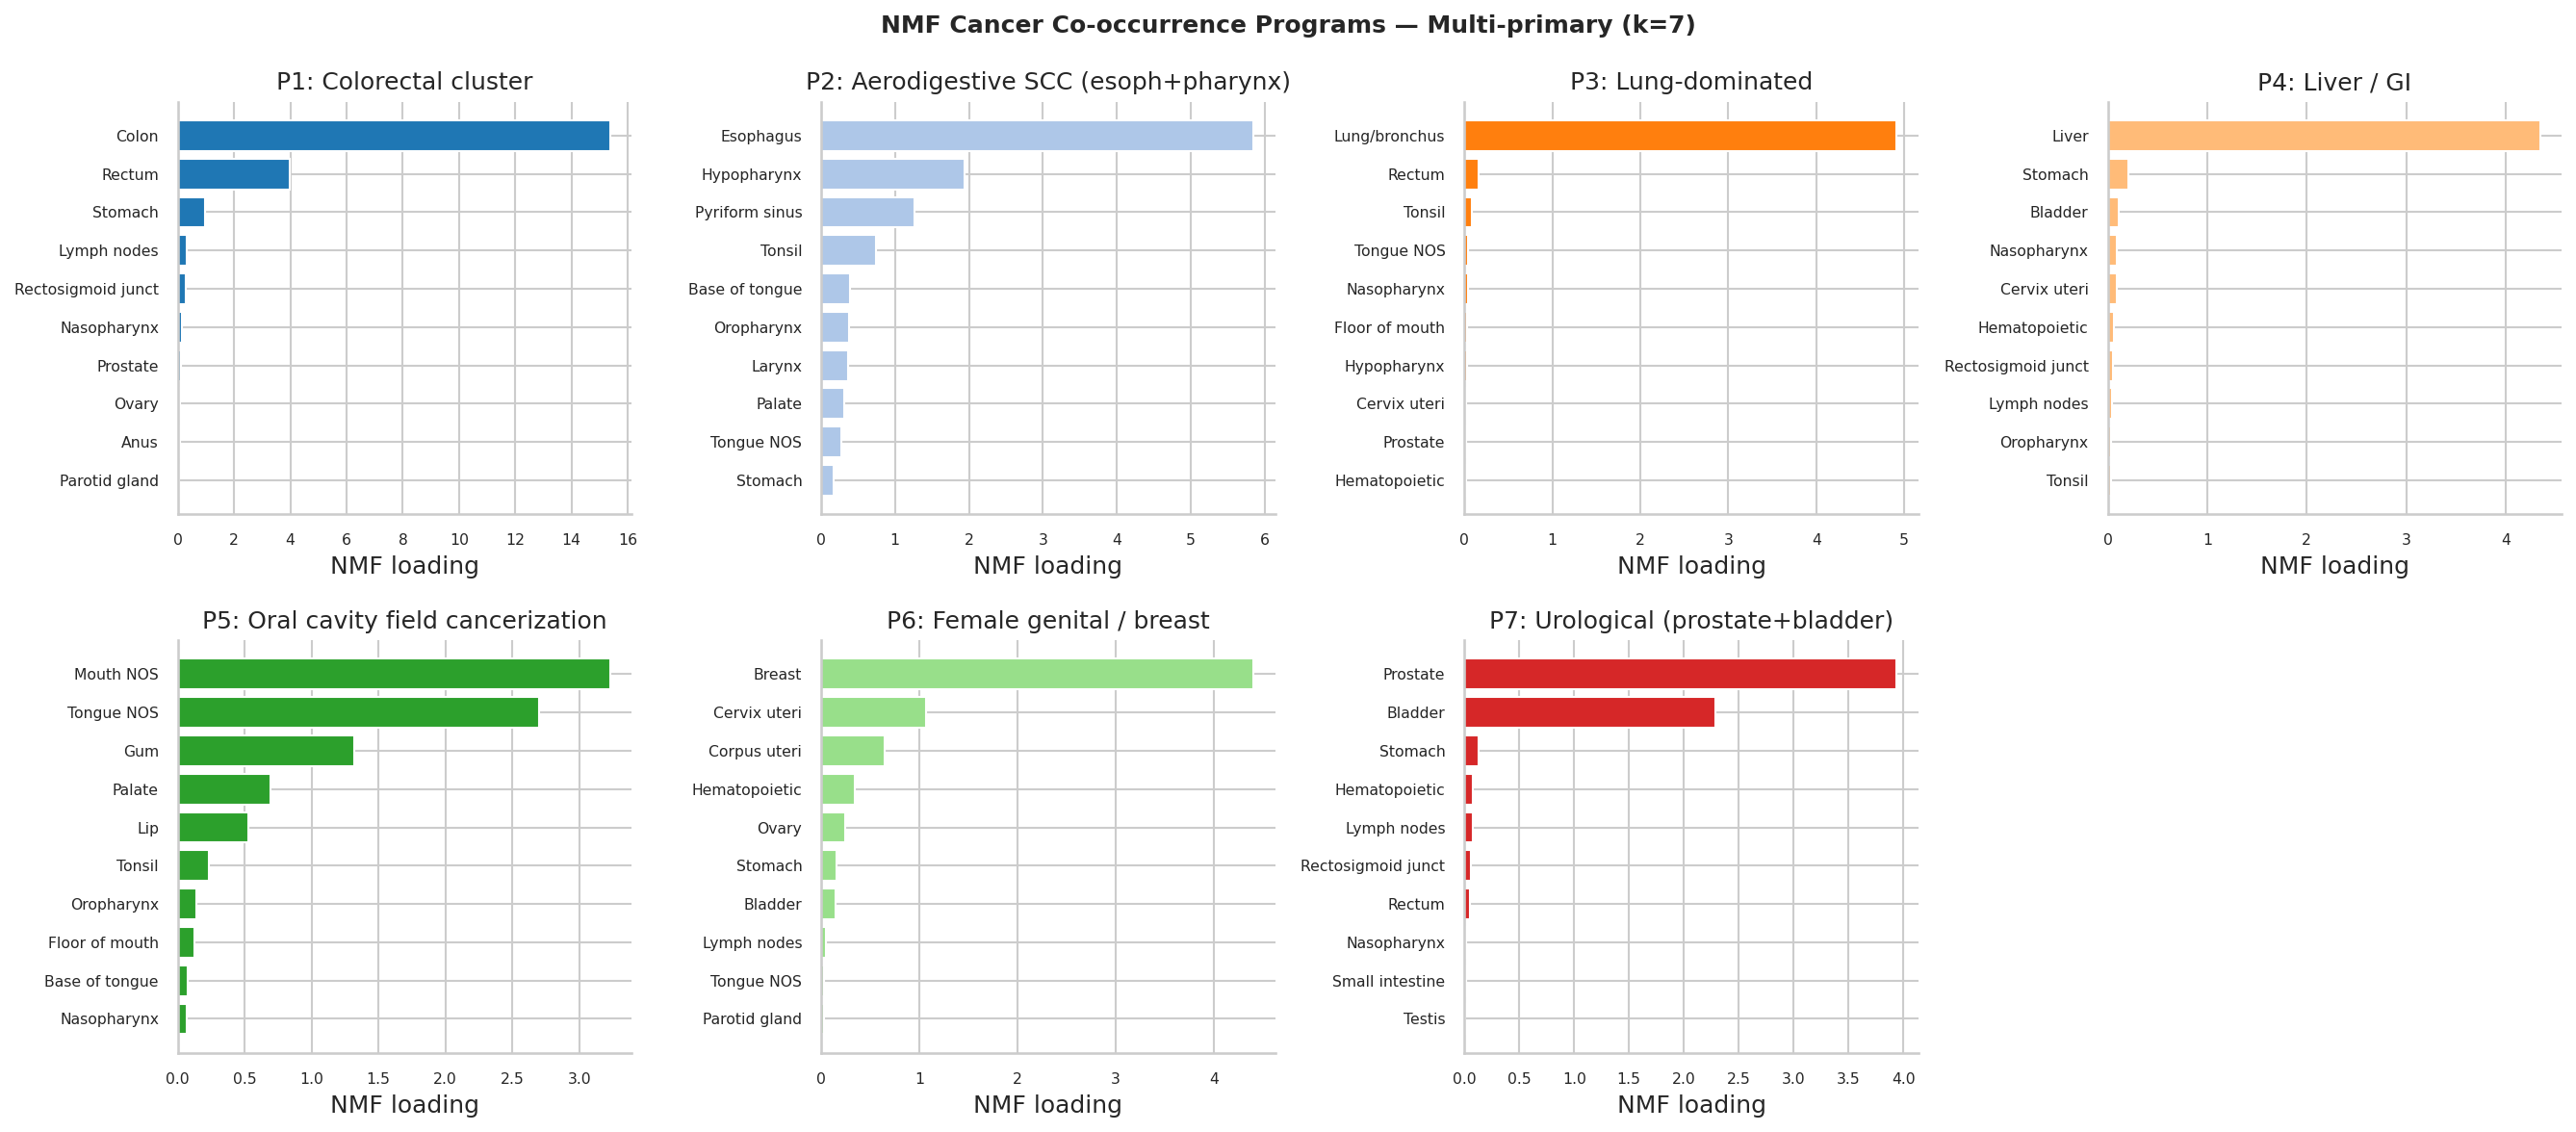
\includegraphics[width=0.95\linewidth]{03_nmf/nmf_programs_multiprimary.png}
  \caption{\textbf{NMF cancer co-occurrence programs ($k = 7$, multiple-primary
    cohort).}
    Each panel shows the cancer-site weight profile for one program. P2
    (Aerodigestive SCC) and P5 (Oral cavity field) are near-exclusively male
    (95--97\,\%), present at the youngest ages (52--53 y), and have the highest
    third-cancer rates (17--19\,\%), consistent with field cancerization.
    P6 captures female reproductive-tract and breast cancers; P7 captures
    age-related urological cancers.}
  \label{fig:nmf}
\end{figure}

\clearpage

\begin{figure}[H]
  \centering
  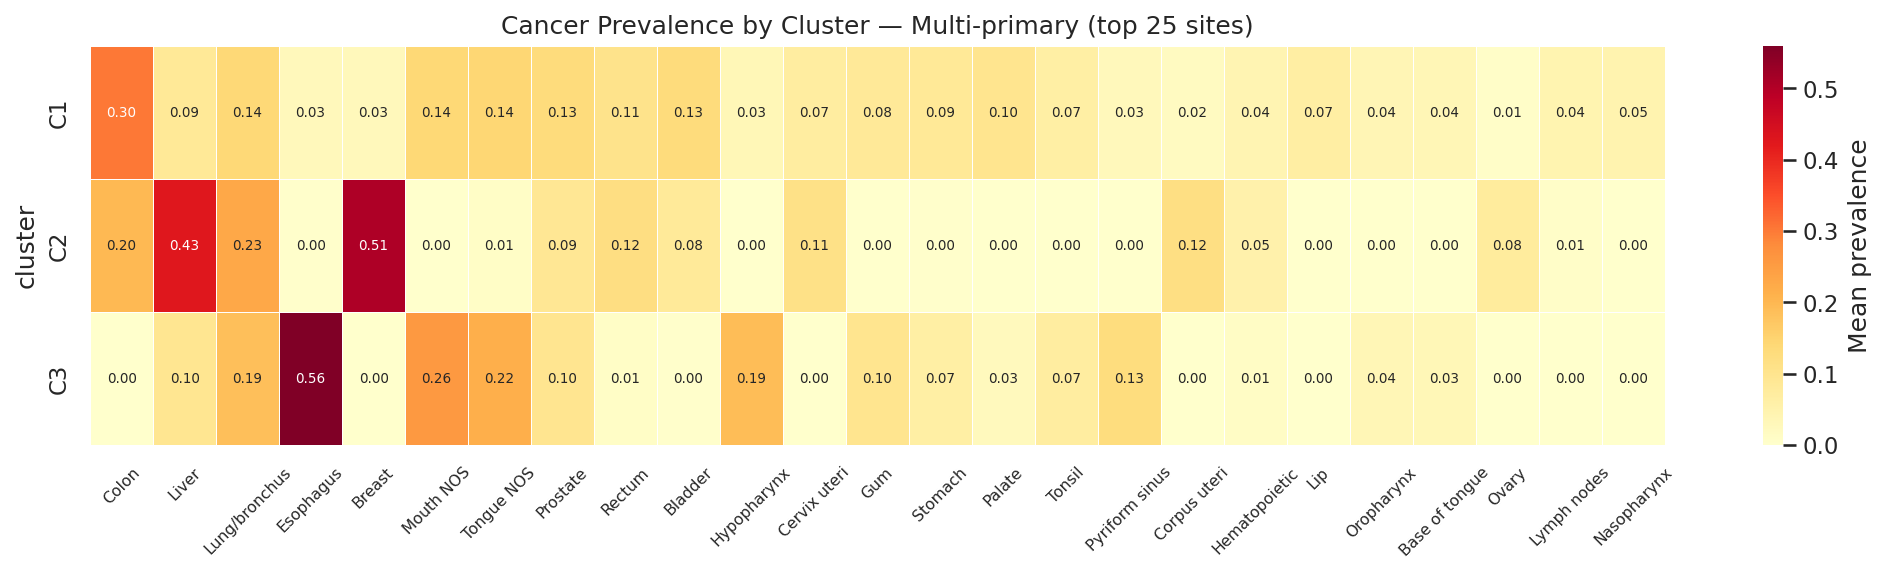
\includegraphics[width=0.92\linewidth]{04_clustering/cluster_cancer_heatmap_k3.png}
  \caption{\textbf{Cancer-site prevalence by autoencoder cluster ($k = 3$).}
    Rows are ICD-O C-code sites; columns are the three clusters. Colour
    intensity encodes the fraction of cluster patients with a diagnosis at that
    site. Cluster~C3 (upper aerodigestive SCC field) shows high prevalence of
    esophagus, hypopharynx, and oral cavity sites; C2 shows breast and
    gynaecological predominance; C1 shows diffuse GI/visceral involvement.}
  \label{fig:clusters}
\end{figure}

\clearpage

\begin{figure}[H]
  \centering
  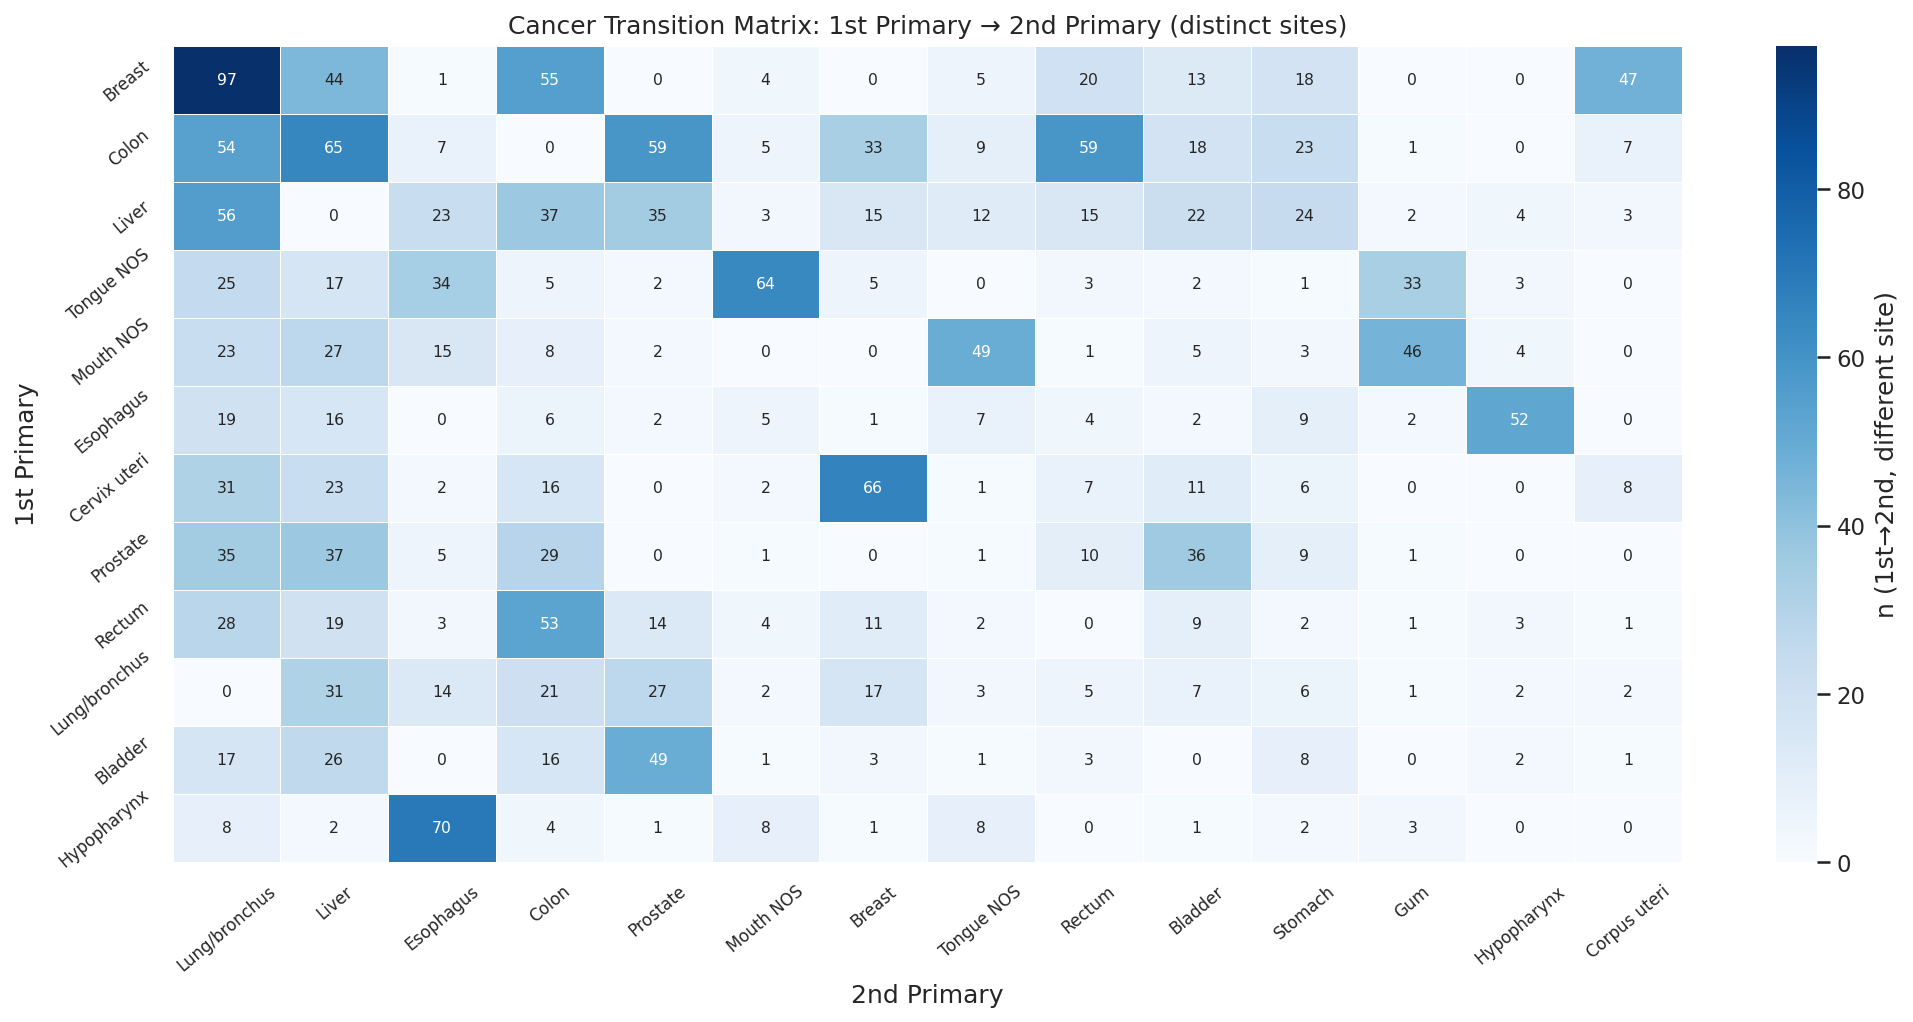
\includegraphics[width=0.85\linewidth]{02_associations/cancer_transition_matrix.png}
  \caption{\textbf{First $\rightarrow$ second primary cancer transition matrix.}
    Each cell encodes the count of patients whose first diagnosed cancer (row)
    was followed by a second at the listed site (column). The bidirectional
    intensity within the upper aerodigestive block (esophagus--hypopharynx--tonsil,
    upper-left quadrant) contrasts with the predominantly unidirectional
    breast\,\textrightarrow\,lung and colon\,\textrightarrow\,liver transitions.}
  \label{fig:transitions}
\end{figure}

\clearpage

\begin{figure}[H]
  \centering
  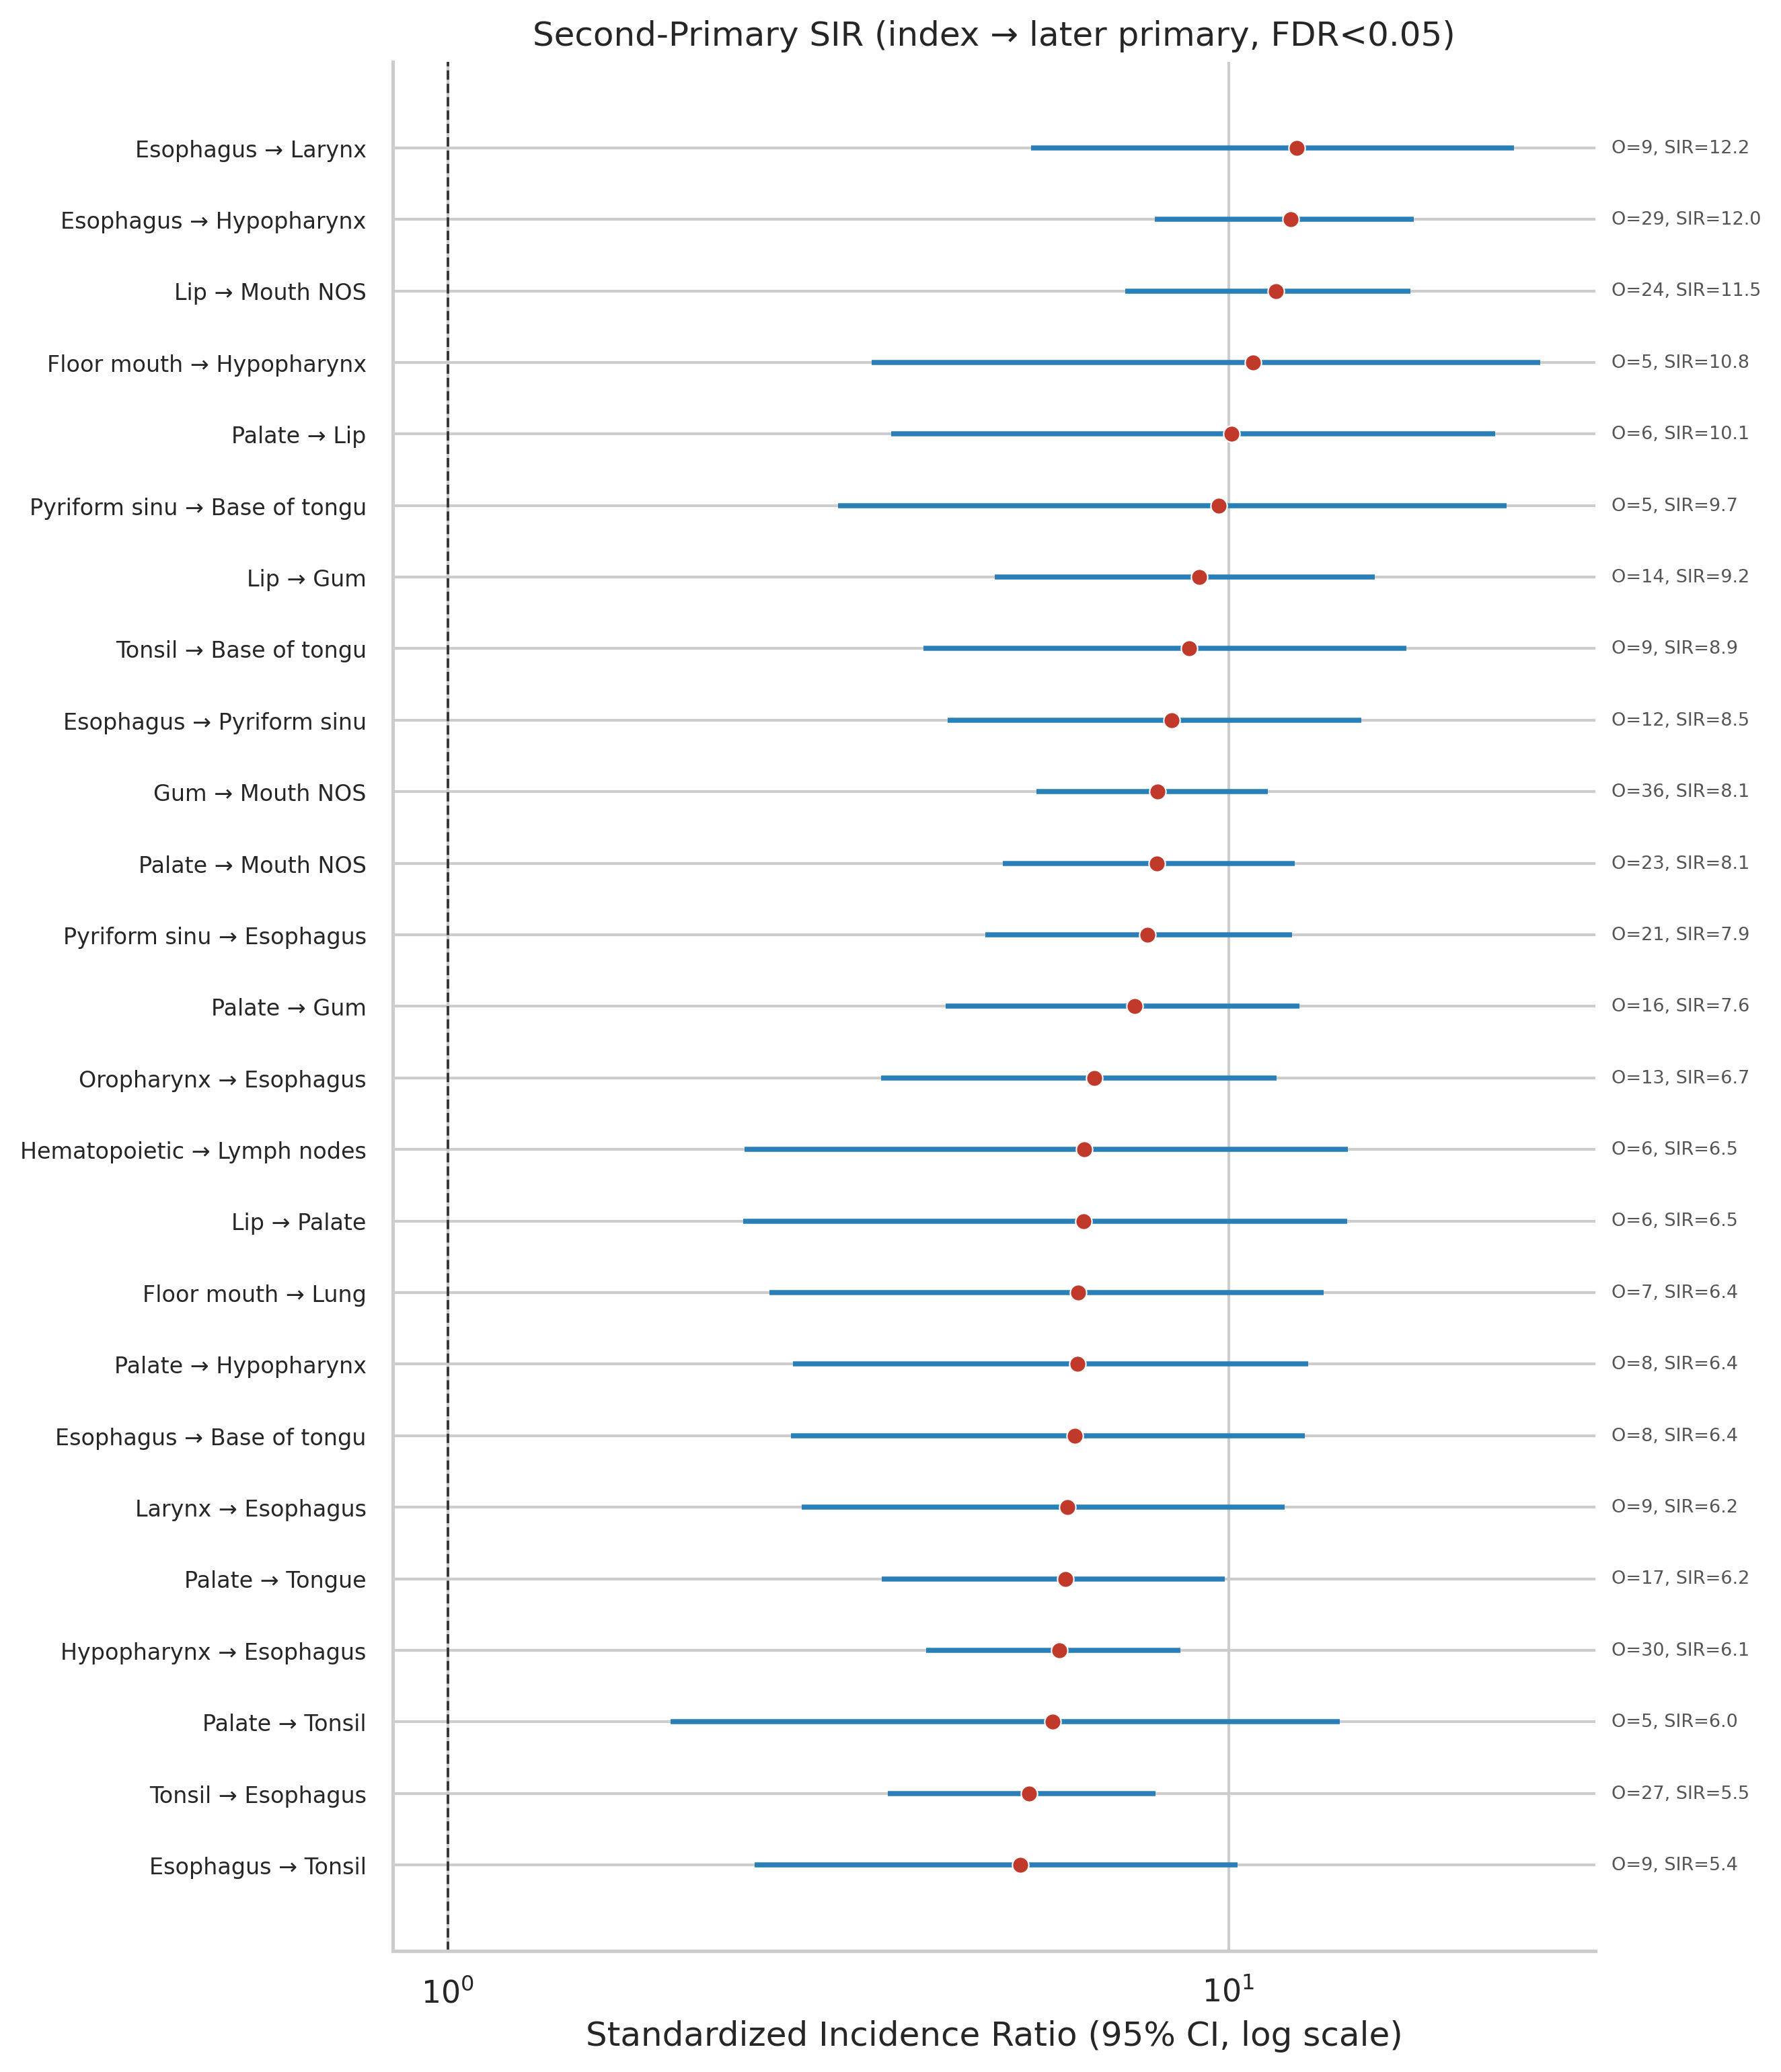
\includegraphics[width=0.88\linewidth]{05_sir_trajectories/sir_forest.png}
  \caption{\textbf{Standardised incidence ratios for second primary cancers
    (FDR $<$ 0.05).}
    Forest plot of SIR with 95\,\% Poisson confidence intervals for the 69
    index\,\textrightarrow\,target pairs that reached FDR $<$ 0.05 after
    Benjamini--Hochberg correction. The highest SIR values are confined to the
    upper aerodigestive field: esophagus\,\textrightarrow\,larynx (SIR 12.2) and
    esophagus\,\textrightarrow\,hypopharynx (SIR 12.0). Dashed line at SIR $=$ 1
    denotes no excess risk.}
  \label{fig:sir}
\end{figure}

\clearpage

\begin{figure}[H]
  \centering
  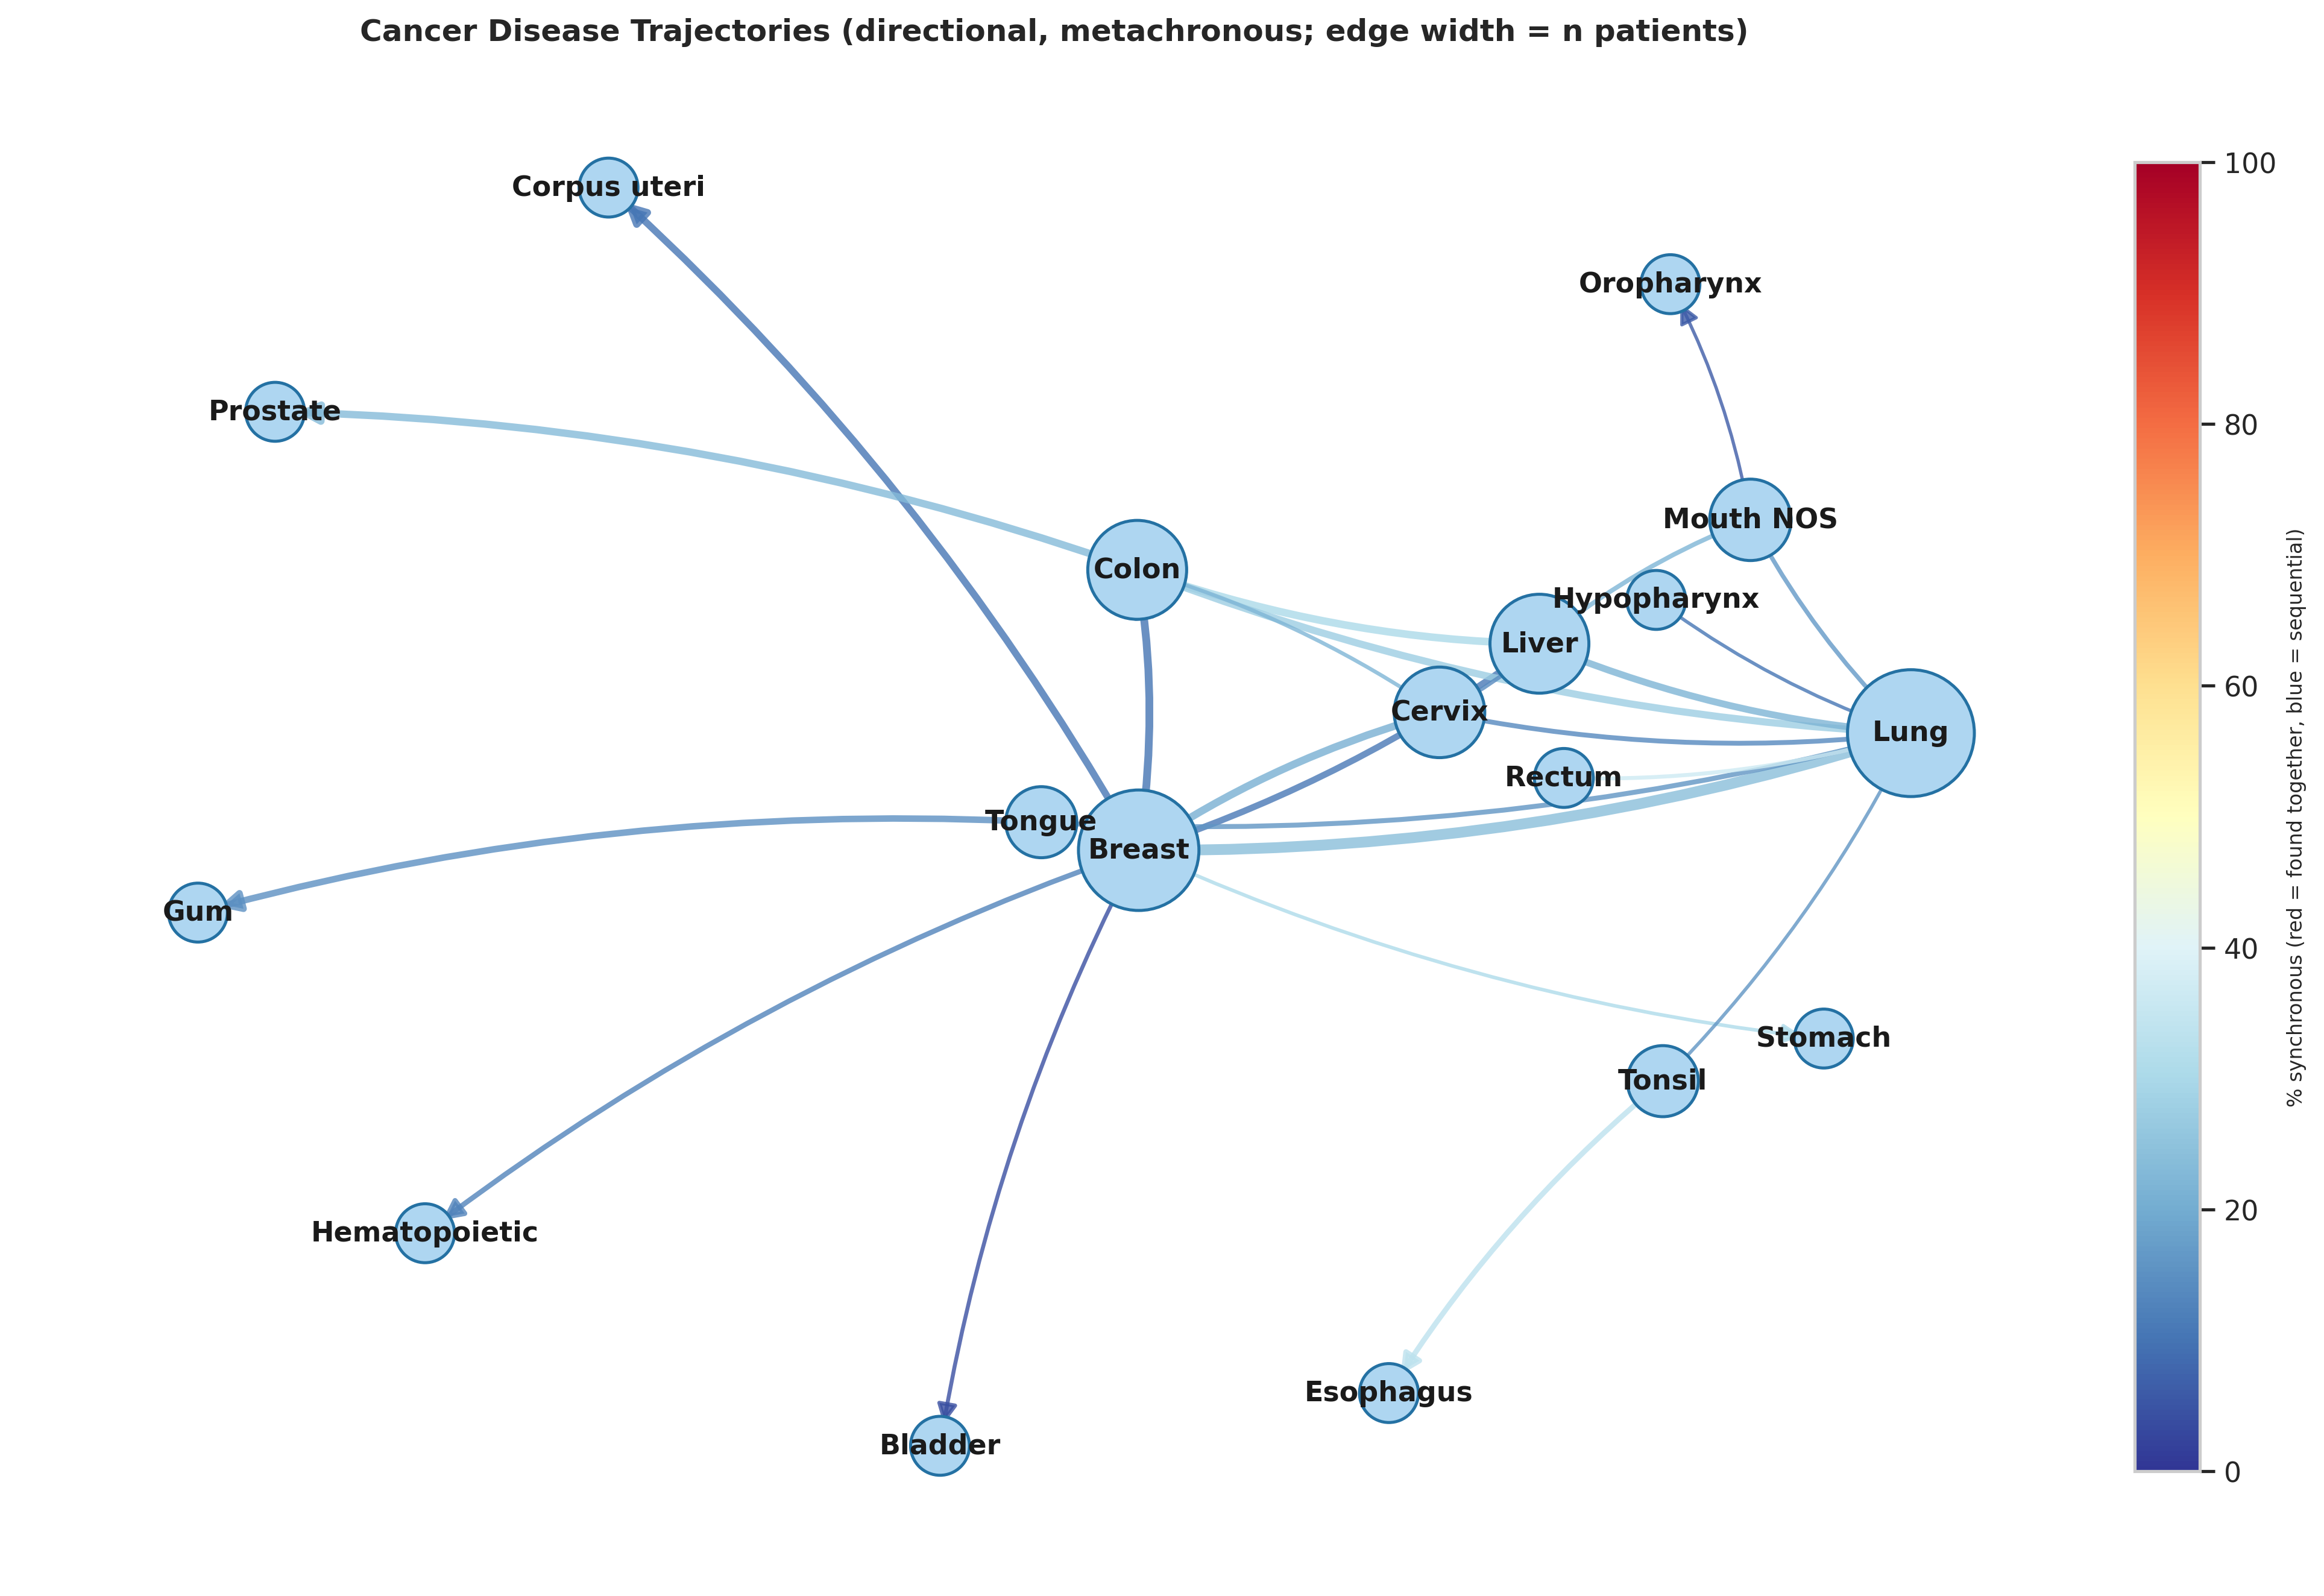
\includegraphics[width=0.88\linewidth]{05_sir_trajectories/trajectory_graph.png}
  \caption{\textbf{Directional disease-trajectory graph.}
    Nodes represent cancer sites; directed edges denote significantly directional
    second-primary sequences (binomial FDR $<$ 0.05). Edge colour encodes the
    percentage of pairs classified as synchronous ($\leq 6$ months); edge weight
    encodes pair count. Aerodigestive pairs (upper cluster) are bidirectional
    (grey, non-significant direction) with predominantly synchronous presentation,
    whereas breast and colorectal second primaries (lower-right) show strong
    unidirectional, metachronous flow.}
  \label{fig:trajectories}
\end{figure}

%%======================================================================
%% Tables
%%======================================================================

\clearpage

\begin{table}[H]
  \centering
  \caption{NMF cancer program clinical profiles (multiple-primary cohort,
    $n = 4{,}068$). Programs are ordered by male percentage.}
  \label{tab:nmf}
  \begin{tabular}{llrrrr}
    \toprule
    Program & Theme & $n$ & Male\,\% & Median age & $\geq$3 cancers\,\% \\
    \midrule
    P2 & Upper aerodigestive SCC  & 615  & 97 & 53 & 17 \\
    P5 & Oral cavity field        & 758  & 95 & 52 & 19 \\
    P7 & Urological               & 406  & 90 & 72 &  5 \\
    P3 & Lung-dominant            & 483  & 74 & 64 &  8 \\
    P4 & Liver/GI                 & 766  & 69 & 64 &  7 \\
    P1 & Colorectal               & 310  & 57 & 64 &  2 \\
    P6 & Female genital/breast$^*$& 730  &  5 & 56 &  3 \\
    \bottomrule
    \multicolumn{6}{p{0.80\textwidth}}{\small Median age = median age at first
      diagnosis (years). $^*$P6: Male\,\% = 5 (i.e., 95\,\% female).
      Mortality\,\% from registry vital status at last contact.}
  \end{tabular}
\end{table}

\clearpage

\begin{table}[H]
  \centering
  \caption{Autoencoder cluster clinical profiles ($k = 3$, $n = 4{,}068$
    multiple-primary patients). Clusters are labelled by dominant cancer domain.}
  \label{tab:clusters}
  \begin{tabular}{llrrrrrr}
    \toprule
    Cluster & Domain & $n$ & Median age & Male\,\% & Mortality\,\% &
    $\geq$3 cancers\,\% \\
    \midrule
    C3 & Aerodigestive SCC field   & 1{,}071 & 55 & 96 & 68.8 & 13 \\
    C1 & GI/visceral mixed         & 1{,}827 & 61 & 76 & 58.8 & 11 \\
    C2 & Female-enriched/breast    & 1{,}170 & 61 & 30 & 49.1 &  4 \\
    \bottomrule
    \multicolumn{7}{l}{\small Mortality\,\% = proportion dead at last registry
      contact (not actuarial survival).}
  \end{tabular}
\end{table}

\clearpage

\begin{table}[H]
  \centering
  \caption{Disease-trajectory directionality and synchronous/metachronous split
    for selected cancer pairs. Forward and Reverse counts reflect metachronous
    directional pairs; \% sync = proportion of all pairs (including synchronous)
    diagnosed within 6 months.}
  \label{tab:trajectories}
  \begin{tabular}{lrrrll}
    \toprule
    Trajectory pair & Forward & Reverse & \% sync & Temporal mode &
    Dir.\ FDR \\
    \midrule
    Hypopharynx $\leftrightarrow$ Esophagus  &  33 & 29 & 60 &
      Field --- synchronous  & ns \\
    Esophagus $\leftrightarrow$ Larynx       &  12 &  9 & 46 &
      Field --- mixed        & ns \\
    Breast $\rightarrow$ Lung                &  90 & 10 & 24 &
      Sequential             & $<$0.001 \\
    Breast $\rightarrow$ Corpus uteri        &  51 & 10 & 10 &
      Sequential             & $<$0.001 \\
    Colon $\rightarrow$ Liver$^\dagger$       &  57 & 22 & 30 &
      Sequential             & 0.002 \\
    Cervix $\rightarrow$ Breast              &  57 & 22 & 21 &
      Sequential             & 0.002 \\
    Colon $\rightarrow$ Prostate             &  55 & 21 & 23 &
      Sequential             & 0.002 \\
    \bottomrule
    \multicolumn{6}{p{0.85\textwidth}}{\small Dir.\ FDR: Benjamini--Hochberg-corrected
      binomial directional test; ns = FDR $\geq$ 0.05 (not significantly directional).
      Forward/Reverse: counts of ordered metachronous pairs;
      \% sync includes synchronous pairs in denominator.
      $^\dagger$The colon$\,\rightarrow\,$liver trajectory may include colorectal
      liver metastases coded as synchronous primaries; sensitivity analysis
      excluding this pair did not alter conclusions regarding upper aerodigestive
      field dominance.}
  \end{tabular}
\end{table}

\end{document}
